\documentclass[TOTEM]{cern/cernphprep}

\usepackage{color}
\usepackage{enumitem}

%----------------------------------------------------------------------------

\def\d{{\rm d}}
\def\un#1{\,{\rm #1}}
\def\ung#1{\quad[{\rm #1}]}
\def\unt#1{[{\rm #1}]}
\def\e{{\rm e}}
\def\I{{\rm i}}
\def\T{{\rm T}}
\def\vec#1{\mathbf{#1}}
\def\mat#1{\mathsf{#1}}
\def\etal{et al.}
\def\todo#1{{\color{red}TODO: #1}}
\def\TODO#1{{\color{red}TODO: #1}}

\setbox123\hbox{$0$}
\setbox124\hbox{$.$}
\def\S{\hbox to\wd123{\hss}}
\def\.{\hbox to\wd124{\hss}}

\def\Name#1{#1, }
\def\Review#1#2#3#4{{\it #1} {\bf #2} (#3) #4}

\def\hang{\hangindent=\parindent}
\catcode`\>=11
\newskip\itskip \itskip2mm
\newskip\iitskip \iitskip0mm
\newdimen\itindent \itindent3mm
\newdimen\iitindent \iitindent5mm
\def\>{\par\vskip\itskip\parindent\itindent\indent\hang\llap{\hbox to3mm{$\bullet$\hss}}}
\def\>E{\par\vskip\itskip\parindent\itindent\indent\hang\llap{\hbox to3mm{\hss}}}
\def\>>{\par\vskip\iitskip\parindent\iitindent\indent\hang\llap{\hbox to\iitindent{\hss--\ }}}

%----------------------------------------------------------------------------------------------------

\begin{document}

\begin{titlepage}

\renewcommand{\EXPLOGO}{fig/logo_totem_black.pdf}

\PHnumber{TODO}
\PHdate{TODO}

\EXPnumber{TODO}
\EXPdate{TODO}

\title{Alignment of CT-PPS detectors in 2016}

\ShortTitle{Alignment of CT-PPS detectors in 2016}

\author{Jan Ka\v spar}

\ShortAuthor{Jan Ka\v spar}



\begin{abstract}
TODO: abstract
\end{abstract}
\end{titlepage}

%----------------------------------------------------------------------------------------------------

\section{Introduction}
\label{s:intro}

\> why is the alignment important
\>> what is the desired precision

\> layout and naming of RPs

\begin{figure}[h!]
\begin{center}
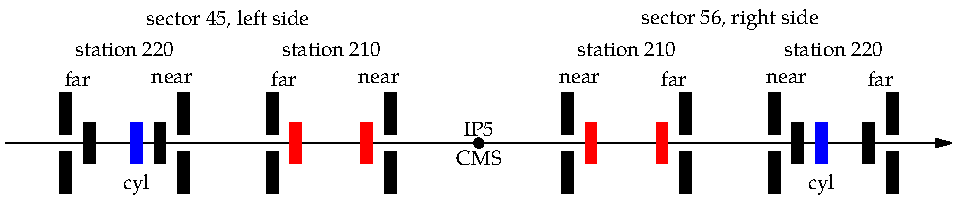
\includegraphics{fig/rp_layout.pdf}
\caption{%
Layout of RPs aroud IP5. The red RPs contain the tracking Si strips sensors used for CT-PPS. The blue RPs host the timing diamond sensors. The other RPs are used only by the TOTEM experiment.
}
\label{fig:rp_layout}
\end{center}
\end{figure}

\> outline of the approach and the structure of the note
\>> two types of runs: calibration, physics

\> two periods -- two alignments
\>> before TS2: calibration run in fill 4828
\>> after TS2: calibration run in fill 5322

%----------------------------------------------------------------------------------------------------

\section{Alignment in calibration runs}
\label{s:calib}

\> calibration run: low intensity, both horizontal and vertical RPs inserted, all RPs close to the beam (\TODO{number of sigmas})

\> the standard ``TOTEM'' procedure -- Section 3.4 in \cite{totem-ijmp}

\> three steps
\>> beam-based alignment: prior to data-taking, RPs are moved to the same $n_\sigma$ distance as collimators, when RPs touch the sharp beam edge created by collimators, strong BLM signal is observed; see Figure 7 in \cite{totem-ijmp}
\>> track-based alignment: relative alignment among all silicon sensors, analysis of track-hit residuals; Section~\ref{s:calib-track}
\>> elastic-based alignment: absolute alignment wrt.~beam, using symmetries of elastic scattering; Section~\ref{s:calib-elastic}

%--------------------------------------------------
\subsection{Relative alignment among RP sensors}
\label{s:calib-track}

\> can use any track passing through the RP station

\> key point: overlap between horizontal and vertical RPs $\rightarrow$ relative alignment among all RPs

\begin{figure}[h!]
\begin{center}
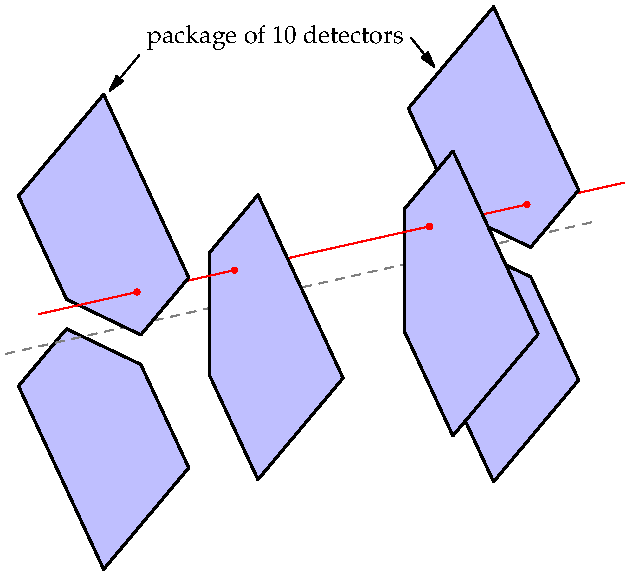
\includegraphics[width=5cm]{fig/rp_overlap.pdf}
\caption{%
A track (red line) passing through an overlap between vertical and horizontal RPs. The blue areas represent stacks of 10 Si strip sensors. The dashed black line indicates the beam.
}
\label{fig:rp_overlap}
\end{center}
\end{figure}

\> general method: analysis of track-hit residuals, see details in Section 4.2 in \cite{jan_thesis}
\>> optimisation of shift (in read-out direction) and rotation (about beam axis) of each Si sensor
\>> performed in several iterations (about 5), gradually imposing more strict track selection cuts as alignment precision improves
\>> not sensitive to certain (global) alignment modes (addressed in Section \ref{s:calib-elastic}): x and y shift and rotation of each unit (near or far) $\rightarrow$ optimising under constraint of zero mean global alignments
\>> applied to several sub-samples (TOTEM runs) for stability and systematics control

\> specific features
\>> 1 or 2 RPs missing in the right arm $\rightarrow$ complications, worse precision, even when using uMuMvRot=true

\> results can be decomposed into
\>> ``RP alignments'': alignments shared by all sensors in a RP
\>> ``internal alignments'': sensors alignments wrt.~the ``RP alignments''

\> examples
\>> Figure \ref{fig:tb_residuals}: residuals become centred about 0 during the procedure
\>> Figure \ref{fig:tb_example_internal}: example of ``internal alignments'', very good stability
\>> Figure \ref{tb_example_rp}: example of ``RP alignments'', very good stability

\begin{figure}[h!]
\begin{center}
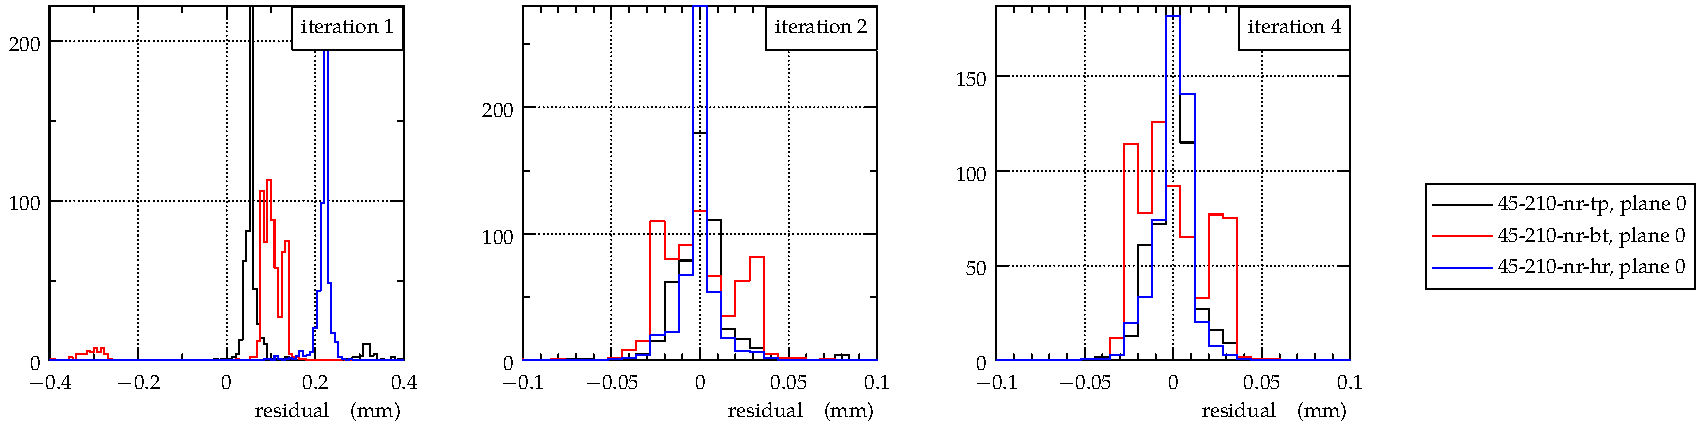
\includegraphics[width=\hsize]{fig/after_TS2/residuals.pdf}
\caption{%
Distributions of track-hit residuals (TOTEM run 10332, after TS2). Each colour corresponds to a different sensor (first planes in the RPs of the 45-210-nr unit). The blue histogram has been downscaled by factor 100. {\it Left}: before any optimisation. The disconnected histogram portions originate from different RP configurations contributing to the fit. {\it Middle}: after shift optimisation. {\it Right}: after shift and rotation optimisation.
}
\label{fig:tb_residuals}
\end{center}
\end{figure}

\begin{figure}[h!]
\begin{center}
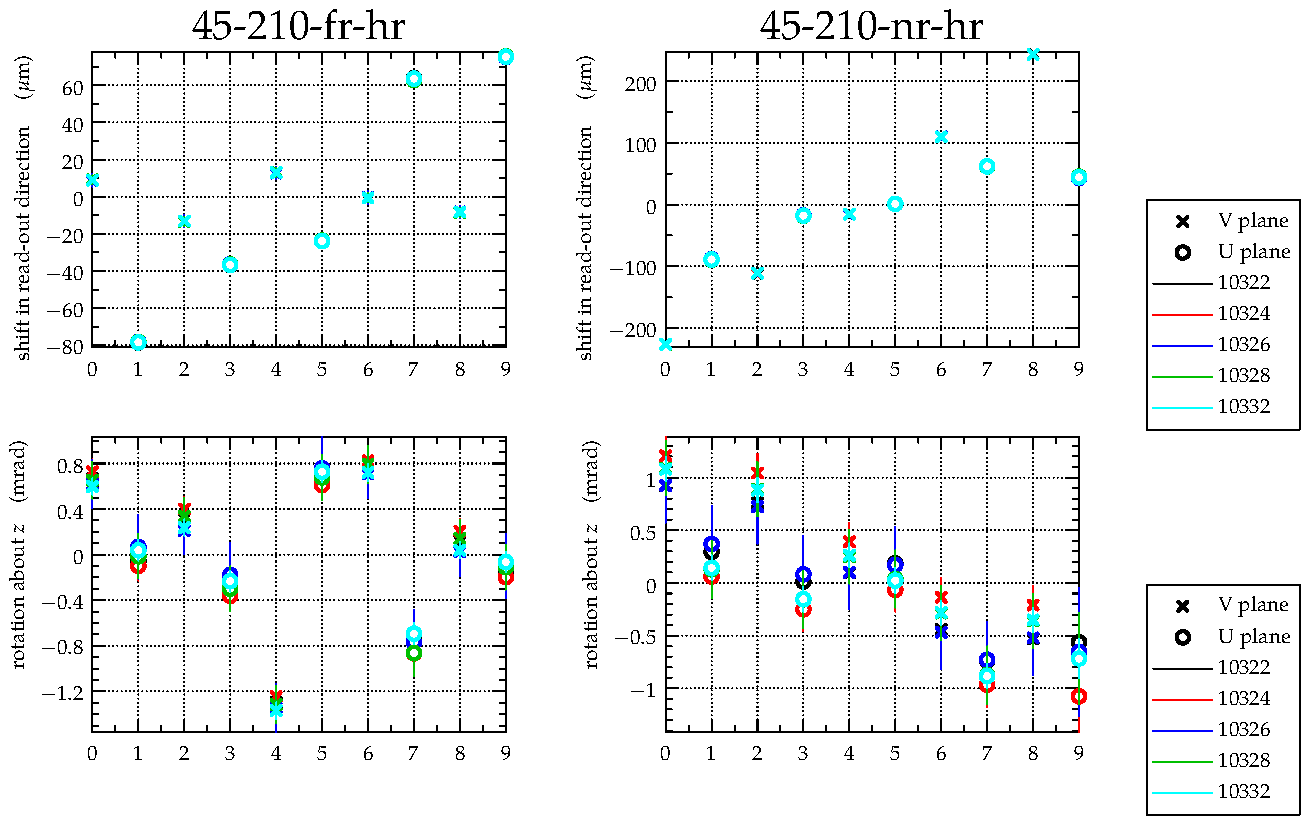
\includegraphics[width=\hsize]{fig/after_TS2/plots_per_plane_left.pdf}
\caption{%
Comparison of internal alignments obtained from different TOTEM runs (different colours), for the period after TS2. The two columns correspond to the two horizontal RPs in the sector 45. The horizontal scale gives the plane index within the detector package: 0 is the closest to the IP, 9 the farthest. The results for ``V'' (``U'') planes are marked with crosses (circles). The linear patterns in the determined shifts (separately in ``U'' and ``V'' projections) can be understood by tilts of the entire detector package which shift the sensor centre's proportionally to its position within the package, for more details see Section 4.2.8 in \cite{jan_thesis}. The error bars indicate statistical uncertainties only.
}
\label{fig:tb_example_internal}
\end{center}
\end{figure}

\begin{figure}[h!]
\begin{center}
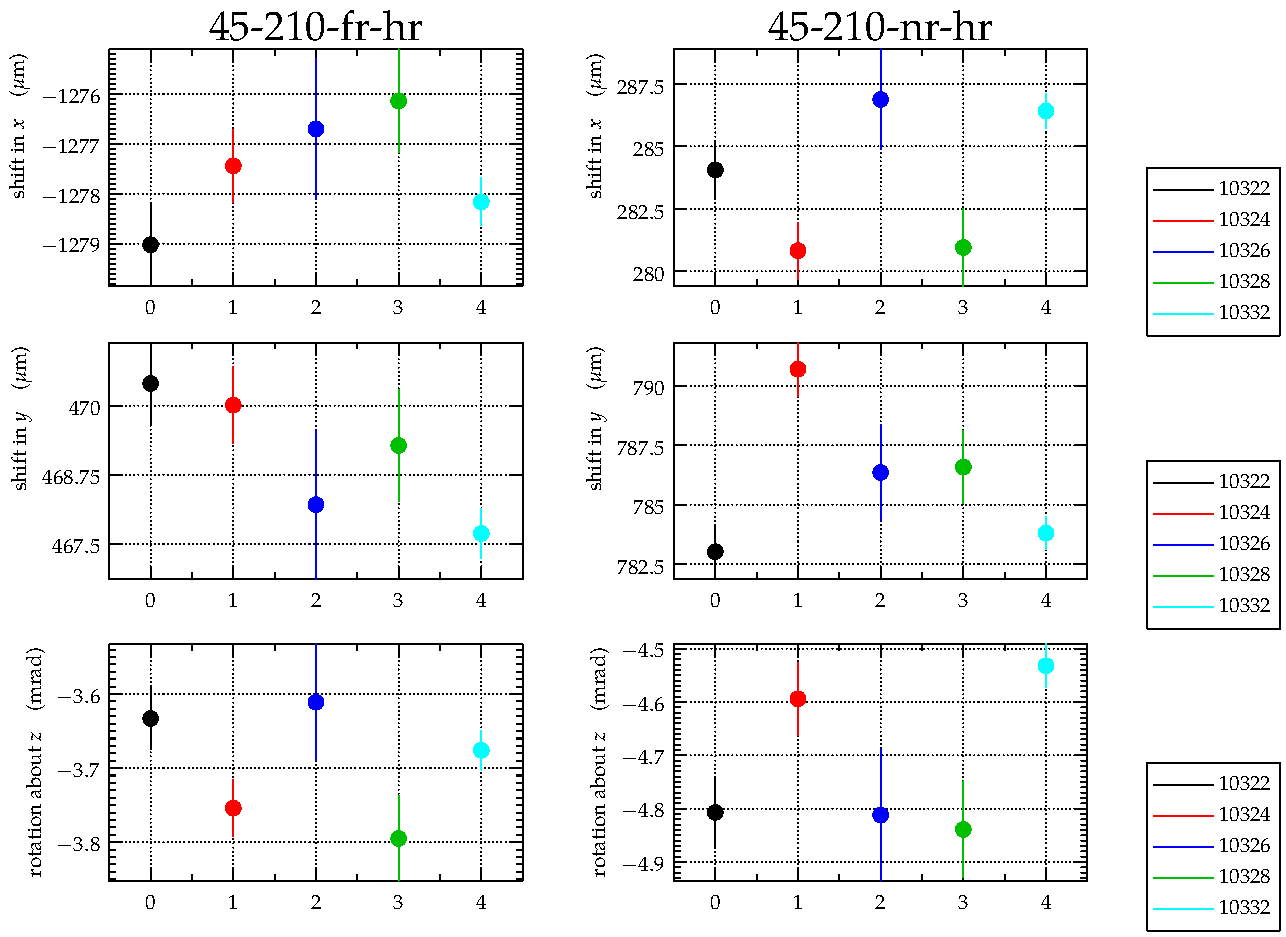
\includegraphics[width=\hsize]{fig/after_TS2/plots_per_rp_left.pdf}
\caption{%
Comparison of ``RP'' alignments obtained from different TOTEM runs (different colours), for the period after TS2. The two columns correspond to the two horizontal RPs in the sector 45. The error bars indicate statistical uncertainties only.
}
\label{fig:tb_example_rp}
\end{center}
\end{figure}


\> uncertainties
\>> statistical uncertainties estimated by the algorithm
\>> systematic uncertainties inferred from the difference between sub-samples, see Figures \ref{fig:tb_example_internal} and \ref{fig:tb_example_rp}.
\>> combined uncertainties:
\>> before TS2 -- \TODO{values}
\>> after TS2 -- left arm: $5\un{\mu m}$ for shifts, $0.3\un{mrad}$ for rotations, right arm: $25\un{\mu m}$ for shifts, $1\un{mrad}$ for rotations 


%--------------------------------------------------
\subsection{Absolute alignment with respect to the beam}
\label{s:calib-elastic}

%----------------------------------------------------------------------------------------------------

\section{Alignment in physics runs}
\label{s:phys}

%----------------------------------------------------------------------------------------------------

\section{Alignment validation}
\label{s:val}

%----------------------------------------------------------------------------------------------------

\section{Summary}
\label{s:sum}

%----------------------------------------------------------------------------------------------------

\begin{thebibliography}{99}

\bibitem{totem-jinst}
	\Name{G.~Anelli \etal{}~(TOTEM Collaboration)}
	\Review{JINST}{3}{2008}{S08007}.
    %The TOTEM Experiment at the CERN Large Hadron Collider, JINST 3 S08007, 2008

\bibitem{plb43}
	\Name{U.~Amaldi et al.}
	\Review{Phys.~Lett.~B}{43}{1973}{231 -- 236}.

\bibitem{jan_thesis}
	\Name{J.~Ka\v spar}
	PhD Thesis, CERN-THESIS-2011-214,
	\url{http://cdsweb.cern.ch/record/1441140}.

\bibitem{totem-ijmp}
	\Name{G.~Antchev \etal{}~(TOTEM Collaboration)}
	\Review{Int.~J.~Mod.~Phys.~A}{28}{2013}{1330046}.

\end{thebibliography}

\end{document}
